%
% Permission is granted to copy, distribute and/or modify this
% document under the terms of the Creative Common by-nc-sa License
% version 3.0 (CC BY-NC-SA 3.0). A copy of the license can be found at
% http://creativecommons.org/licenses/by-nc-sa/3.0/legalcode.
%

\usepackage[french]{babel}
\usepackage{multicol}
\usepackage{fancyvrb}
\fvset{fontsize=\footnotesize}
\RecustomVerbatimEnvironment{verbatim}{Verbatim}{}
\usetikzlibrary{patterns}

% Highlight macros
\newcommand{\highlight}[1]{\textcolor{structure.fg}{\bfseries #1}}

%% Title, subtitle, authors, institute, date, ...
\title{Analyse de malware statique et dynamique}
\subtitle{Les outils et quelques cas pratiques}

\author[E. Grelet \& A. Guémon]{Erwan Grelet \& Amélie Guémon\\[1em]}

%\author[E. Grelet \& A. Guémon]{Erwan Grelet \& Amélie Guémon\\[1em]
%  \texttt{\scriptsize <erwan.grelet@etu.u-bordeaux.fr>}\\[.3em]
%  \texttt{\scriptsize <amelie.guemon@etu.u-bordeaux.fr>}}

\institute[Master CSI, France]{Master CSI, Université de Bordeaux, France}

\date{\today}

%%%%%%%%%%%%%%%%%%%%%%%%%%[ Document ]%%%%%%%%%%%%%%%%%%%%%%%%%%
\begin{document}

\begin{frame}
  \vspace{3.5em}
  \titlepage
  \begin{center}
    
\includegraphics[scale=.2]{cc-by-nc-sa.pdf}
  \end{center}
\end{frame}
%%%%%%%%%%%%%%%%%%%%%%%%%%%%%%%%%%%%%%%%%%%%%%%%%%%%%%%%%%%%%%%%%%%%%%
\section*{Introduction}

\begin{frame}[fragile]
  \frametitle{Introduction}
  \vspace{-.5em}
  Quelques statistiques \ldots
  \vfill
  \begin{itemize}\setlength\itemsep{1.5em}
        \item{58.31\% des emails échangés durant l'année 2016 étaient des spams,
        \\soit 3 points de plus qu'en 2015;}
        %https://securelist.com/analysis/kaspersky-security-bulletin/77483/kaspersky-security-bulletin-spam-and-phishing-in-2016/
        \item{Plus de 90\% des emails de phishing contenaient des ransomwares;}
        %sur le premier semestre 2016
        \item{En 2016, 1 088 900 victimes de banking trojans,
        30\% de plus qu'en 2015;}
        %https://securelist.com/analysis/publications/77623/financial-cyberthreats-in-2016/
        %\item{notamment pokémongo Trojan-Banker.AndroidOS.Tordow et guide ztorg
        \item{En septembre 2016, attaque DDOS de 1 Tb/s
        sur les serveurs d'OVH France;}
        %depuis IoT (152 464 caméras, routeurs, thermostats, \ldots
        \item{Code source du botnet Mirai disponible.}
        %avec scanner de vulnérabilité d'IoT intégré, \ldots
  \end{itemize}
  \vspace{-.25em}
\end{frame}
% ###################################################%
\begin{frame}[fragile]
  \frametitle{Introduction}
  \begin{multicols}{2}[{\large Quelques types de menaces:}]
  \begin{itemize}\setlength\itemsep{1.5em}
        \item{Adware;}
        \item{Spyware;}
        \item{Worm;}
        \item{Trojan;}
        \item{Rootkit;}
        \item{Backdoors;}
        \item{Keyloggers;}
        \item{Rogue security software;}
        \item{Ransomware;}
        \item{Browser Hijacker;}
        \item{Botnet;}
        \item{\ldots}
  \end{itemize}
  \end{multicols}
  \vspace{-.25em}
\end{frame}
% ###################################################%
\begin{frame}
  \frametitle{Plan}
  \tableofcontents[]
\end{frame}
%%%%%%%%%%%%%%%%%%%%%%%%%%%%%%%%%%%%%%%%%%%%%%%%%%%%%%%%%%%%%%%%%%%%%%
\section{Les Techniques d'Analyses}

\begin{frame}<handout:0>
  \frametitle{Plan}
  \tableofcontents[currentsection]
\end{frame}
%###################################################%
\begin{frame}[fragile]
  \frametitle{Les Techniques d'Analyses}
\vspace{-.25em}
\begin{itemize}\setlength\itemsep{2.5em}
        \uncover<1-3>{\item{Analyse statique: étude du binaire suspect sans l'exécuter;}}
        \uncover<2-3>{\item{Analyse dynamique: étude au cours de l'exécution et de l'infection;}}
        \uncover<3-3>{\item{Analyse mémoire: étude l'image mémoire après infection.}}
        %obtenir post-mortem info comme process, connection net,
        %code, injections, API hooking, load kernel modules, \ldots
\end{itemize}
\end{frame}
%###################################################%
\begin{frame}[fragile]
  \frametitle{Les Techniques d'Analyses -- Statique}
  \vspace{-.25em}
  \begin{itemize}
    \item{Examen de l'exécutable:\\
      \begin{figure}[H]
      \begin{verbatim}
$> readelf -h ch23
En-tête ELF:
  Magique:   7f 45 4c 46 01 01 01 00 00 00 00 00 00 00 00 00
  Classe:                            ELF32
  Données:                           complément à 2, système à octets de
poids faible d'abord (little endian)
  Version:                           1 (current)
  OS/ABI:                            UNIX - System V
  Version ABI:                       0
  Type:                              EXEC (fichier exécutable)
  Machine:                           Intel 80386
  Version:                           0x1
  Adresse du point d'entrée:         0x8048450
  Début des en-têtes de programme :  52 (octets dans le fichier)
  Début des en-têtes de section :    2404 (octets dans le fichier)
  [...]
\end{verbatim}
\caption {Données comprises dans l'en-tête d'un binaire ELF}
\end{figure}
   }
 \end{itemize}
\end{frame}
%###################################################%
\begin{frame}[fragile]
  \frametitle{Les Techniques d'Analyses -- Statique}
  \vspace{-.25em}
  \begin{itemize}
    \item{Recherche de chaînes de caractères:\\
\begin{figure}[H]
\begin{verbatim}[fontsize=\scriptsize]
$> /tmp/HB3$ strings ch23
/lib/ld-linux.so.2
__gmon_start__
libc.so.6
_IO_stdin_used
strncpy
__stack_chk_fail
printf
strlen
memset
__libc_start_main
Usage : %s <your name>
.init
.text
.data
.bss
main
_init
\end{verbatim}
\caption{Résultat partiel de la commande \textit{strings} sur un binaire}
\end{figure}
}
  \end{itemize}
\end{frame}
%###################################################%
\begin{frame}[fragile]
  \frametitle{Les Techniques d'Analyses -- Statique}
  \vspace{-.25em}
  \begin{itemize}
    \item{Protections du binaire:\\[1.5em]
      \begin{columns}
        \begin{column}{0.4\textwidth}
          $\bullet$ Binaire stripped;\\
          $\bullet$ Détection de débugueur;\\
          $\bullet$ Anti-virtualisation (VM);\\
        \end{column}
        \begin{column}{0.3\textwidth}  %%<--- here
          $\bullet$ Anti-dumping;\\
          $\bullet$ Anti-tampering;\\
          $\bullet$ Packing;\\
        \end{column}
      \end{columns}
      \vspace{1cm}
     \begin{figure}[H]
       \centering
       \begin{tikzpicture}[scale=0.6]
       \draw[line width=.8pt] (0,0) -- (0,.8) -- (4,.8) -- (4,0) --cycle;
       \draw[line width=.8pt, pattern=checkerboard, pattern color=red!70]
       (1,0) -- (1,.8) -- (4,.8) -- (4,0) --cycle;
       \draw[<->, >=latex] (0,-.2) -- (1,-.2);
       \node[align=center] at (0.5,-.8){\footnotesize \shortstack{routine de\\déchiffrement}};
       \draw[->, >=latex] (0.65,.8) [out=90, in=90] to (2,.8);
       \node[align=center] at (1.7,1.9){
       \footnotesize \shortstack{déchiffre l'intégralité\\ du payload restant}};

       \draw[line width=.8pt] (9,0) -- (9,.8) -- (15,.8) -- (15,0) --cycle;
       \draw[line width=.8pt, pattern=checkerboard, pattern color=red!70]
       (10,0) -- (10,.8) -- (15,.8) -- (15,0) --cycle;
       \draw[line width=.8pt, fill=blue!70]
       (12.5,0) -- (12.5,.8) -- (15,.8) -- (15,0) --cycle;
       \draw[pattern=checkerboard, pattern color=red!70]
       (12.5,0) -- (12.5,.8) -- (15,.8) -- (15,0) --cycle;
       \draw[line width=.8pt, dashed] (15,.8) -- (16,.8);
       \draw[line width=.8pt, dashed] (15,0) -- (16,0);
       \draw[<->, >=latex] (9,-.2) -- (10,-.2);
       \node[align=center] at (9.5,-.8){\footnotesize \shortstack{routine de\\déchiffrement}};
       \draw[<->, >=latex] (11.5,-.2) -- (12.5,-.2);
       \node[align=center] at (12,-.8){\footnotesize \shortstack{routine de\\déchiffrement}};
       \draw[->, >=latex] (9.65,.8) [out=90, in=90] to (11,.8);
       \node[align=center] at (9,1.9){
       \footnotesize \shortstack{déchiffre la partie\\ \textcolor{red}{rouge} du payload }};
       \draw[->, >=latex] (12,.8) [out=90, in=90] to (13.5,.8);
       \node[align=center] at (13,1.9){
       \footnotesize \shortstack{déchiffre la partie\\ \textcolor{blue!70}{bleue} du payload}};
     \end{tikzpicture}
     \caption{\label{packer}Différentes formes de packer chiffrant}
   \end{figure}
}
  \end{itemize}
\end{frame}
%###################################################%
\begin{frame}[fragile]
  \frametitle{Les Techniques d'Analyses -- Statique}
  \vspace{-.25em}
  \begin{itemize}
    \item{Lecture de code:\\TODO:Image to post here}
  \end{itemize}
\end{frame}
%###################################################%
\begin{frame}[fragile]
  \frametitle{Les Techniques d'Analyses -- Dynamique}
  \vspace{-.25em}
  \begin{itemize}\setlength\itemsep{2.5em}
    \item{Mise en place de machines virtuelles (VM);}
    \item{Simulation de réseaux (INetSim);}
    \item{Analyse de trafic réseaux. TODO: screenshot}
  \end{itemize}
\end{frame}
%###################################################%
\begin{frame}[fragile]
  \frametitle{Les Techniques d'Analyses -- Dynamique}
  \vspace{-.25em}
  \begin{itemize}\setlength\itemsep{2.5em}
    \item{Étude des processus actifs;}
    \item{Étude des appels systèmes;}
    \item{Débugueur.TODO: screenshots ou code}
  \end{itemize}
\end{frame}
%%%%%%%%%%%%%%%%%%%%%%%%%%%%%%%%%%%%%%%%%%%%%%%%%%%%%%%%%%%%%%%%%%%%%%
\section{BillGates Botnet}

\begin{frame}<handout:0>
  \frametitle{Plan}
  \tableofcontents[currentsection]
\end{frame}
%###################################################%
\begin{frame}[fragile]
  \frametitle{BillGates Botnet -- Miscellaneous}
\vspace{-.25em}
Historique + infection pour IoT
\end{frame}
%###################################################%
\begin{frame}[fragile]
  \frametitle{BillGates Botnet -- Main}
\vspace{-.25em}
Main + cha\^ine obfusqu\'ee
\end{frame}
%###################################################%
\begin{frame}[fragile]
  \frametitle{BillGates Botnet -- Modules}
\vspace{-.25em}
Description Modules + sch\'ema
\end{frame}
%###################################################%
\begin{frame}[fragile]
  \frametitle{BillGates Botnet -- Attaques}
  \vspace{-.25em}
  Types d'attaques mises en place
\end{frame}
%%%%%%%%%%%%%%%%%%%%%%%%%%%%%%%%%%%%%%%%%%%%%%%%%%%%%%%%%%%%%%%%%%%%%%
\section{SageCrypt Ransomware}

\begin{frame}<handout:0>
  \frametitle{Plan}
  \tableofcontents[currentsection]
\end{frame}

%###################################################%
\begin{frame}[fragile]
  \frametitle{SageCrypt Ransomware -- Origine}
  \vspace{-.25em}
  Les influences notables :
  \begin{itemize}
    \item CryLocker
    \item Petya
  \end{itemize}
\end{frame}
%###################################################%
\begin{frame}[fragile]
  \frametitle{SageCrypt Ransomware -- Fonctionnement}
  \vspace{-.10em}
  Mais comment se propagent les ransomwares ?
  \vfill
  \begin{figure}[H]
     \center
     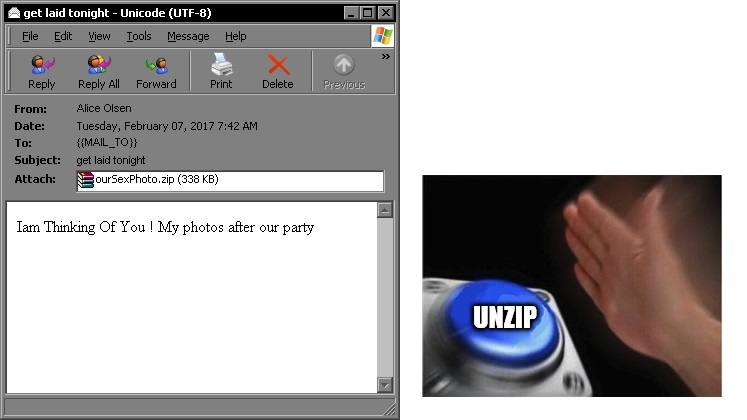
\includegraphics[width=200pt]{dank_meme.jpg}
    \label{fig:mail}
  \end{figure}
\end{frame}
%###################################################%
\begin{frame}[fragile]
  \frametitle{SageCrypt Ransomware -- Fonctionnement}
  \vspace{-.20em}
  Méthodes d'infection classiques
  \vfill
  \begin{itemize}
    \item Emails
    \begin{itemize}
      \item Macros Microsoft Office
      \item Exécutable déguisé
    \end{itemize}
    \item Exploit kits
    \begin{itemize}
      \item Adobe Flash Player
      \item Oracle Java
      \item Apple Quicktime
      \item Mozilla Firefox
    \end{itemize}
  \end{itemize}
\end{frame}
%###################################################%
\begin{frame}
  \frametitle{SageCrypt Ransomware -- Fonctionnement}
  \vspace{-.25em}
  UAC
  \begin{figure}[H]
    \center
    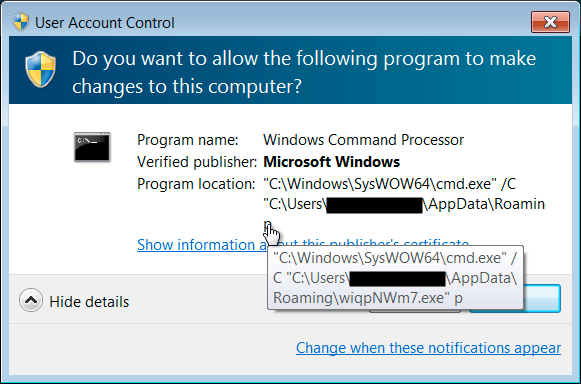
\includegraphics[width=200pt]{uac.jpg}
    \label{fig:uac}
  \end{figure}
\end{frame}
%###################################################%
\begin{frame}
  \frametitle{SageCrypt Ransomware -- Fonctionnement}
  \vspace{-.25em}
  Layout clavier
\end{frame}
%###################################################%
\begin{frame}
  \frametitle{SageCrypt Ransomware -- Fonctionnement}
  \vspace{-.25em}
  Extensions
\end{frame}
%###################################################%
\begin{frame}[fragile]
  \frametitle{SageCrypt Ransomware -- Obfuscation}
  \vspace{-.25em}
  Fonctions / jmp
\end{frame}
%###################################################%
\begin{frame}[fragile]
  \frametitle{SageCrypt Ransomware -- Obfuscation}
  \vspace{-.25em}
  Packing du code
\end{frame}
%###################################################%
\begin{frame}[fragile]
  \frametitle{SageCrypt Ransomware -- Chiffrement}
  \vspace{-.25em}
  Algorithmes utilisés pour le chiffrement :
  \vfill
  \begin{itemize}
    \item Diffie-Hellman basé sur les courbes elliptiques
	\item ChaCha
  \end{itemize}
\end{frame}
%###################################################%
\begin{frame}[fragile]
  \frametitle{SageCrypt Ransomware -- Chiffrement}
  \vspace{-.25em}
  Chiffrement d'un fichier :
  \vfill
  \begin{itemize}
    \item On génère $k_c \in \mathbb{F}_p$ aléatoirement
    \item On calcule le point $Q_c = k_c * G$
    \item On calcule le secret partagé $S = k_c * Q_s = (k_c * k_s) * G$
    \item On dérive du secret partagé, un entier $sh \in \mathbb{F}_p$
    \item On calcule le point $P = sh * G$
    \item On génère $n \in \mathbb{F}_p$ aléatoirement
    \item On calcule les points $chacha\_key = n * P = (n * sh) * G$ et
      $chacha\_pub = n * G$
    \item On chiffre le fichier en utilisant ChaCha avec une clé dérivée de
      $chacha\_key$ 
    \item On ajoute les valeurs de $Q_c$ et $chacha\_pub$ à la fin du fichier
  \end{itemize}
\end{frame}
%###################################################%
\begin{frame}[fragile]
  \frametitle{SageCrypt Ransomware -- Chiffrement}
  \vspace{-.25em}
  En pratique, Sage génère des fichiers qui la structure suivante :
  \vfill
  \begin{figure}[H]
    \center
    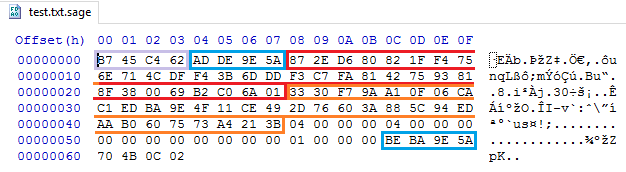
\includegraphics[width=200pt]{dump_file.png}
    \label{fig:file}
  \end{figure}
  Légende :
  \begin{itemize}
  \item Mauve : Contenu chiffré du fichier original
  \item Rouge : $Q_c$
  \item Orange : $chacha\_pub$
  \item Bleu : Valeurs constantes
  \end{itemize}
\end{frame}
%%%%%%%%%%%%%%%%%%%%%%%%%%%%%%%%%%%%%%%%%%%%%%%%%%%%%%%%%%%%%%%%%%%%%%
\section*{Conclusion}

\begin{frame}[fragile]
  \frametitle{Conclusion}
  \vspace{-.25em}
  \begin{columns}
    \begin{column}{0.5\textwidth}
      \begin{itemize}\setlength\itemsep{1.5em}
        \uncover<1-4>{\item{Les malwares sont de structures
        et de caractéristiques très variés;}}
        \uncover<2-4>{\item{Possible automatisation de certaines tâches,
        par le biais de sandbox comme \textit{Cuckoo} ou \textit{Limon};}}
        \uncover<3-4>{\item{Nouvelles formes de classification des malwares (ex: CFG);}}
        \uncover<4-4>{\item{Mais automatisation totale impossible car la
        reconnaissance de malware est un problème indécidable,
        réductible au problème de l'arrêt.}}
      \end{itemize}
    \end{column}
    \begin{column}{0.5\textwidth}
      \centering
      
\includegraphics[scale=0.5]{Pandorre.jpg}
    \end{column}
  \end{columns}
\end{frame}
%%%%%%%%%%%%%%%%%%%%%%%%%%%%%%%%%%%%%%%%%%%%%%%%%%%%%%%%%%%%%%%%%%%%%%
%\section{Références \& Lectures supplémentaires}

%\begin{frame}<handout:0>
%  \frametitle{Plan}
%  \tableofcontents[currentsection,subsectionstyle=hide]
%\end{frame}

%\nocite{*}
%\bibliographystyle{alpha}

%\begin{frame}[allowframebreaks]
%  \frametitle{Livres et références}
%  \bibliography{bibliography}
%\end{frame}

%%%%%%%%%%%%%%%%%%%%%%%%%%%%%%%%%%%%%%%%%%%%%%%%%%%%%%%%%%%%%%%%%%%%%%
\begin{frame}
  \vfill
  \centering
  \highlight{\Huge Questions~?}
  \vfill
\end{frame}
